
\documentclass[9pt]{article}
\usepackage[colorlinks=true, allcolors=blue]{hyperref}
\usepackage[table,xcdraw]{xcolor}
\usepackage[utf8]{inputenc}
\usepackage{graphicx}
\usepackage[colorinlistoftodos]{todonotes}
\usepackage[colorlinks=true, allcolors=blue]{hyperref}
\usepackage{multirow}
\usepackage[spanish]{babel}
\selectlanguage{spanish}
% Esto es para poder escribir acentos directamente:
\usepackage[utf8]{inputenc}
\usepackage[T1]{fontenc}
\usepackage{amssymb}
\usepackage{enumitem}
\usepackage{pifont}
\usepackage{tikz}
\usepackage[latin1]{inputenc}
\usepackage{makeidx}
\makeindex
%% Asigna un tamaño a la hoja y los márgenes
\usepackage[a4paper,top=1.2cm,bottom=1.5cm,left=2cm,right=2cm,marginparwidth=1.75cm]{geometry}
\usepackage{wrapfig}
\usepackage{fancyhdr}
\usepackage{multirow}
\usepackage{caption}
\usepackage{longtable}
\usepackage{gensymb}
\usepackage{float}
\usepackage[position=top]{subfig}
\usepackage{verbatim}
\setlength\parindent{0pt}
%% spce line 
\usepackage{setspace}
	\setstretch{1.1}
\usepackage{pdfpages}
%% Paquetes de la AMS
\usepackage{amsmath, amsthm, amsfonts}
\usepackage{tikz}
\usetikzlibrary{shapes.geometric}
\usetikzlibrary{shapes.arrows}
\usepackage{array} 
\usepackage[dvipsnames]{xcolor}
\usepackage{xcolor}
\usepackage{soul}
\newcommand{\mathcolorbox}[2]{\colorbox{#1}{$\displaystyle #2$}}
\date{}

\begin{document}

\begin{titlepage} % Suppresses displaying the page number on the title page and the subsequent page counts as page 1
	\newcommand{\HRule}{\rule{\linewidth}{0.5mm}} % Defines a new command for horizontal lines, change thickness here
	
	\center % Centre everything on the page
	
	%------------------------------------------------
	%	Headings
	%------------------------------------------------
	
\includegraphics[width=0.7\textwidth]{logoudesa.jpg}\\[0.8cm]
	
	\textsc{\LARGE Herramietas Computacionales para la Investigación}\\[0.5cm] % Major heading such as course name
	
	\textsc{\Large Amelia Gibbons}\\

	%------------------------------------------------
	%	Title
	%------------------------------------------------
	\textcolor{white}{\HRule}\\[0.6cm]
	\huge\bfseries Trabajo Práctico 4
	\textcolor{white}{\HRule}\\[1.5cm]
	%------------------------------------------------
	%	Author(s)
	%------------------------------------------------
	\begin{center}
		\Large
		\textsc{Liwski, Sury}\\
	\end{center}
	
	% If you don't want a supervisor, uncomment the two lines below and comment the code above
	%{\large\textit{Author}}\\
	%John \textsc{Smith} % Your name
	
	%------------------------------------------------
	%	Date
	%------------------------------------------------
	\vfill\vfill\vfill % Position the date 3/4 down the remaining page
	{\large 2022}
	\vfill
	
\end{titlepage}
\section*{Tarea 1}
\subsection*{BMI}
A continuaci\'on se presenta una readaptaci\'on del gr\'afico \texttt{pd4}. Por cuestiones de escala, dado que lo que deseamos corregir es la forma de presentar el gr\'afico, lo realizamos con una subsecci\'on de cuatro pa\'ises. A continuaci\'on el original:
\begin{figure}[H]
    \centering
    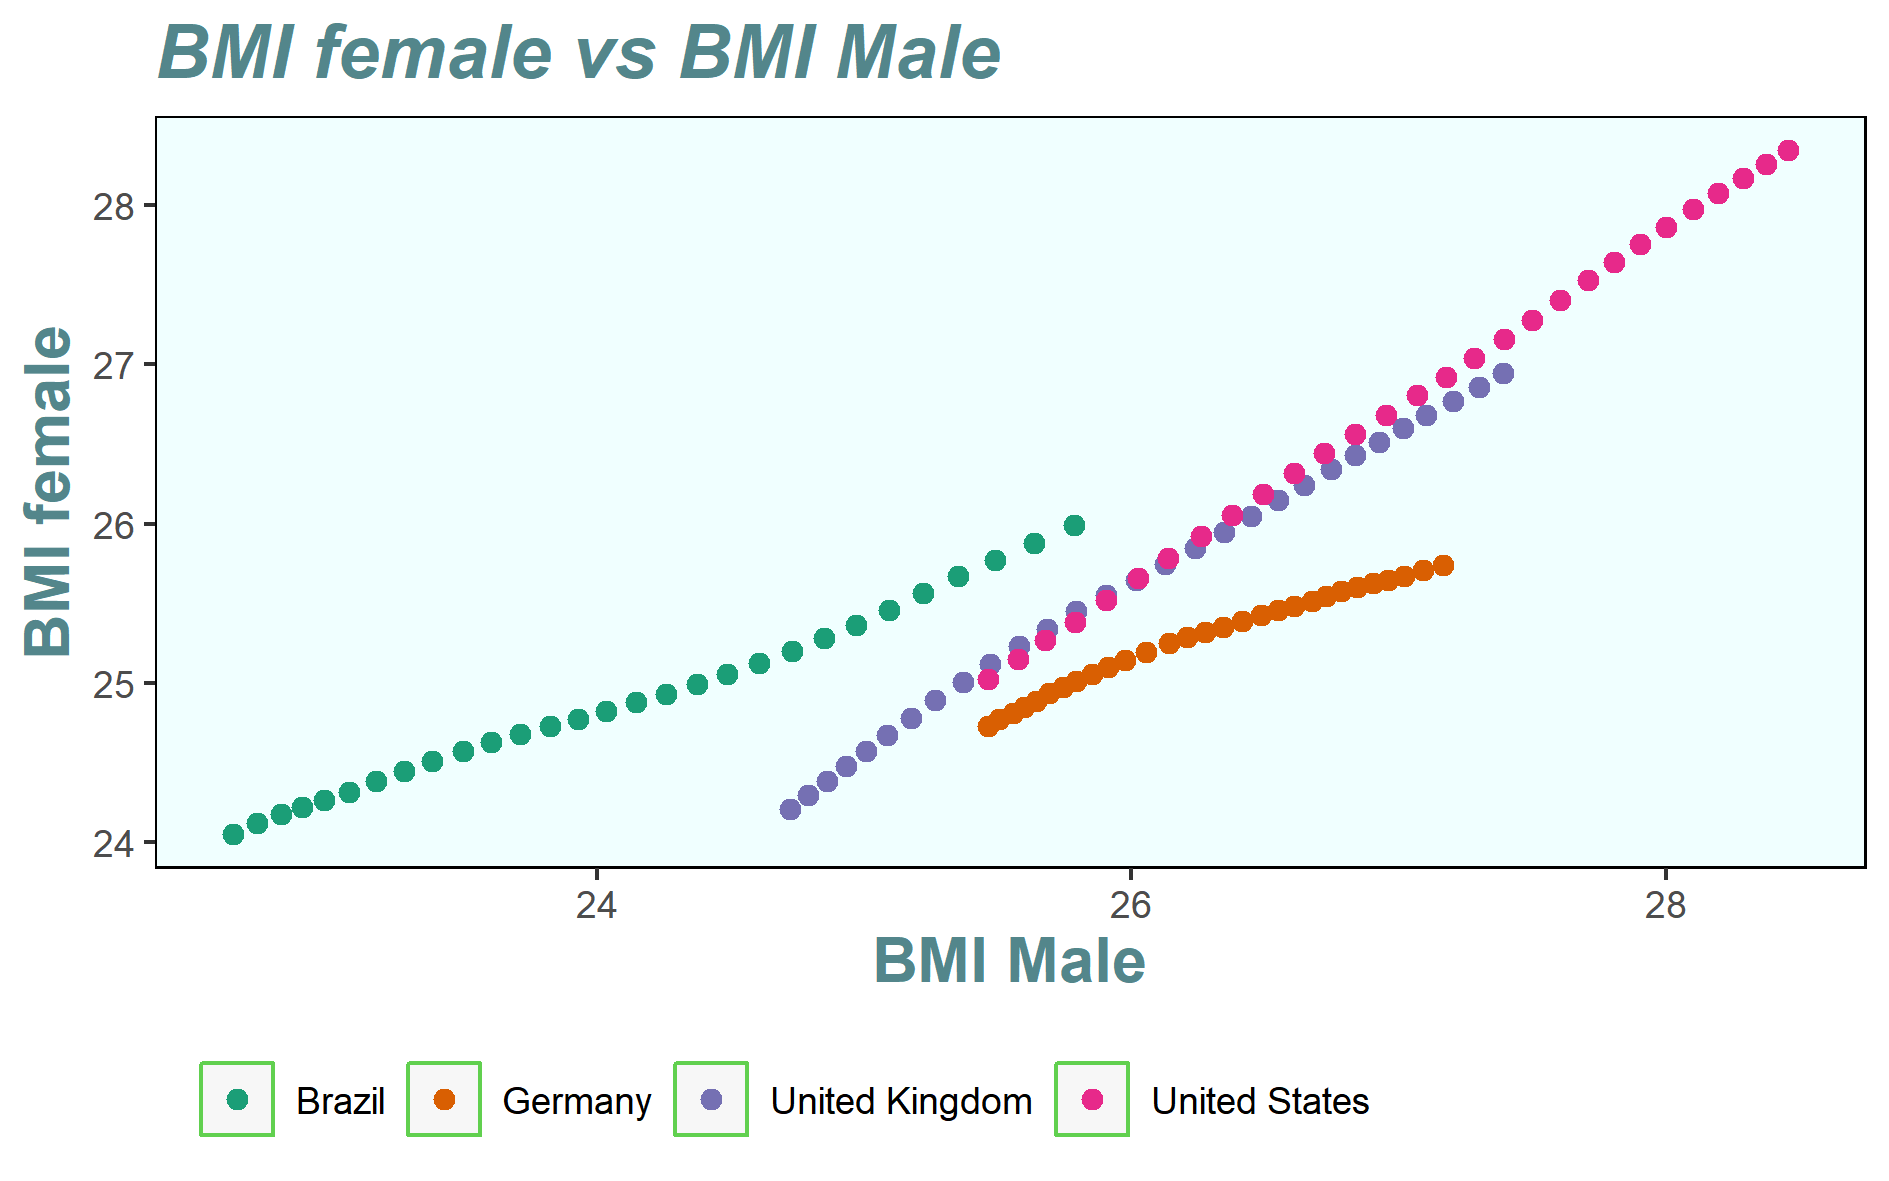
\includegraphics{original3.png}
\end{figure}
Para incluir toda la informaci\'on en el gr\'afico, lo dividimos en \textit{facets}, coloreando en cada una la correspondiente al pa\'is y dejando las dem\'as en gris. Utilizamos un \textit{theme} y paleta de colores que nos result\'aron m\'as est\'etica con la intenci\'on que resulte homog\'enea con los dem\'as gr\'aficos de este inciso.
\begin{figure}[H]
    \centering
    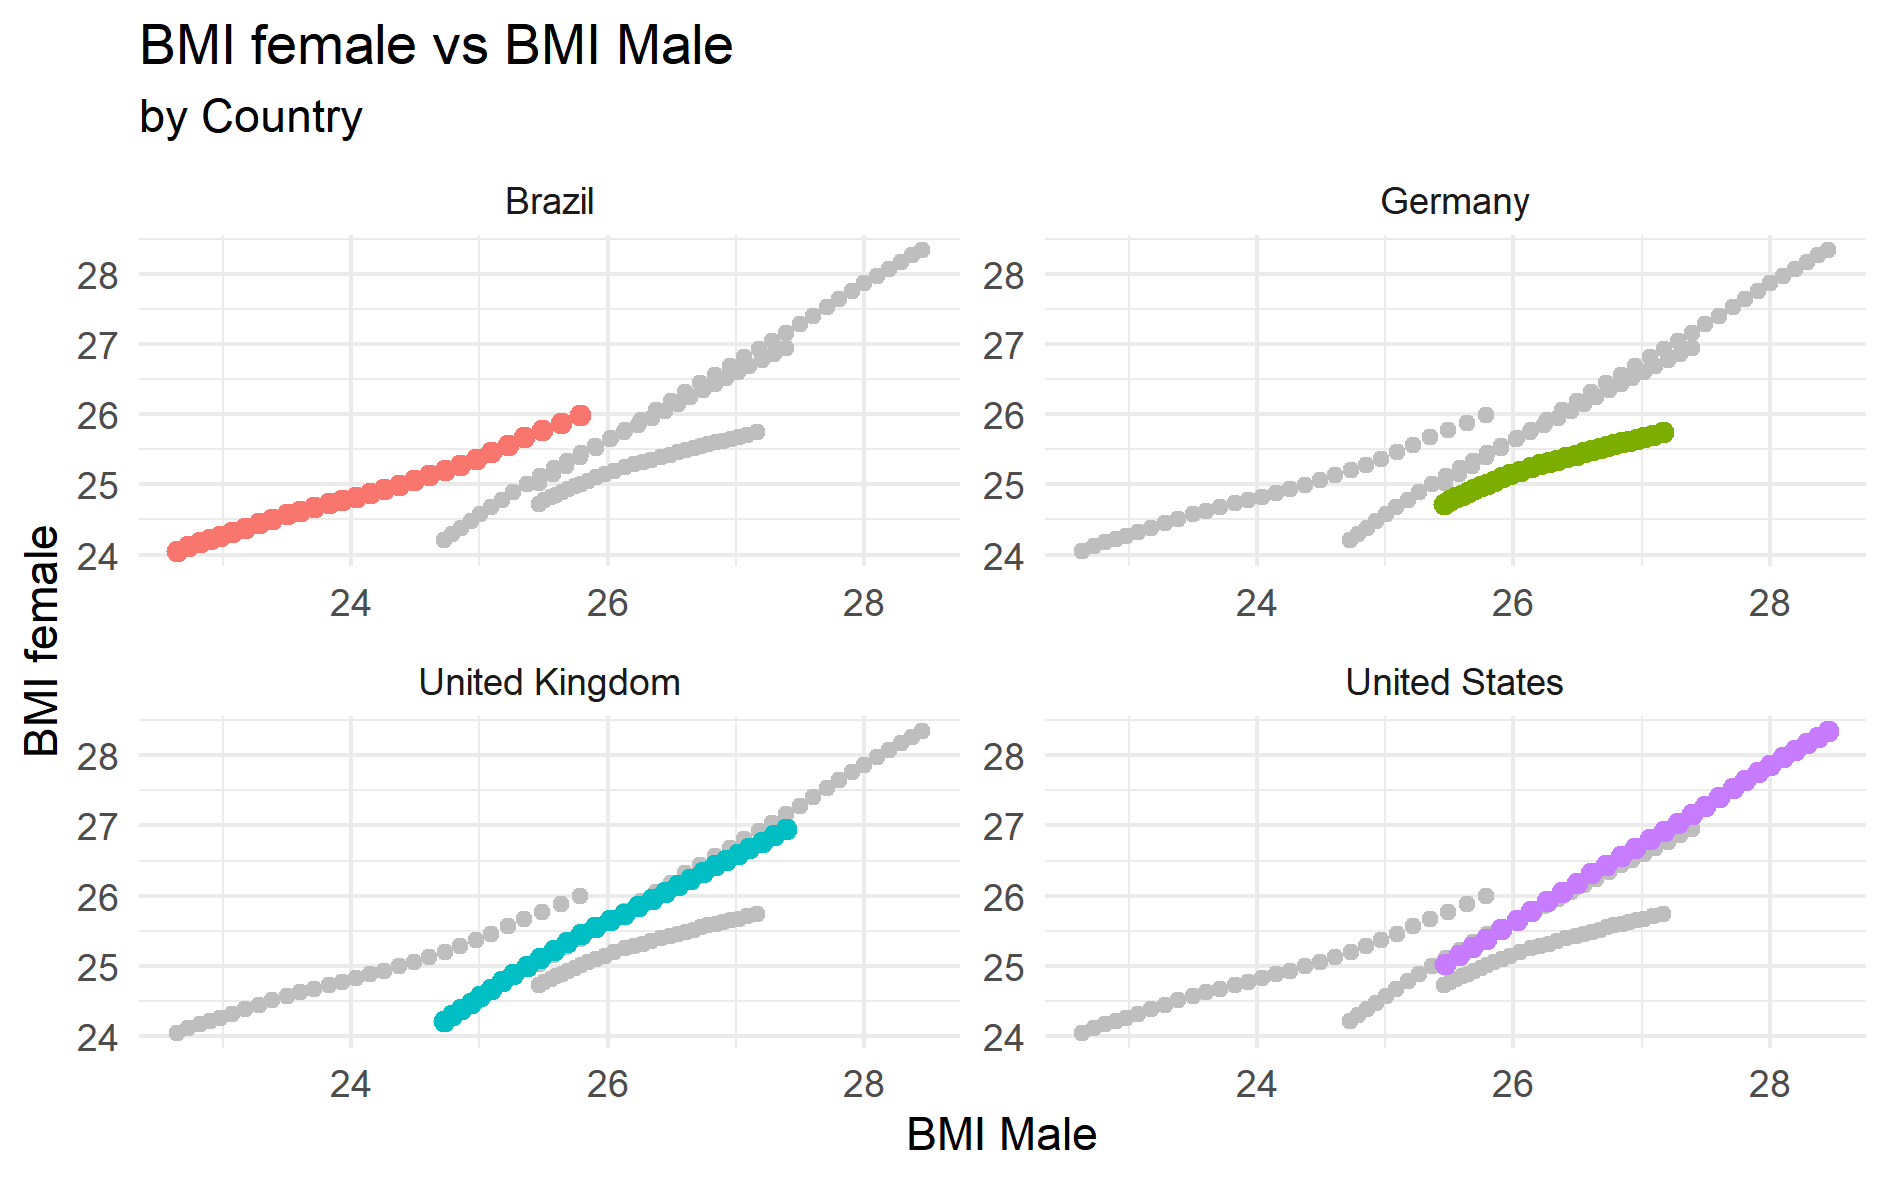
\includegraphics{changed3.png}
\end{figure}
\subsection*{Mapa de Europa}
Utilizando una subselecci\'on de pa\'ises, presentan a continuaci\'on el siguiente mapa de Europa. 
\begin{figure}[H]
    \centering
    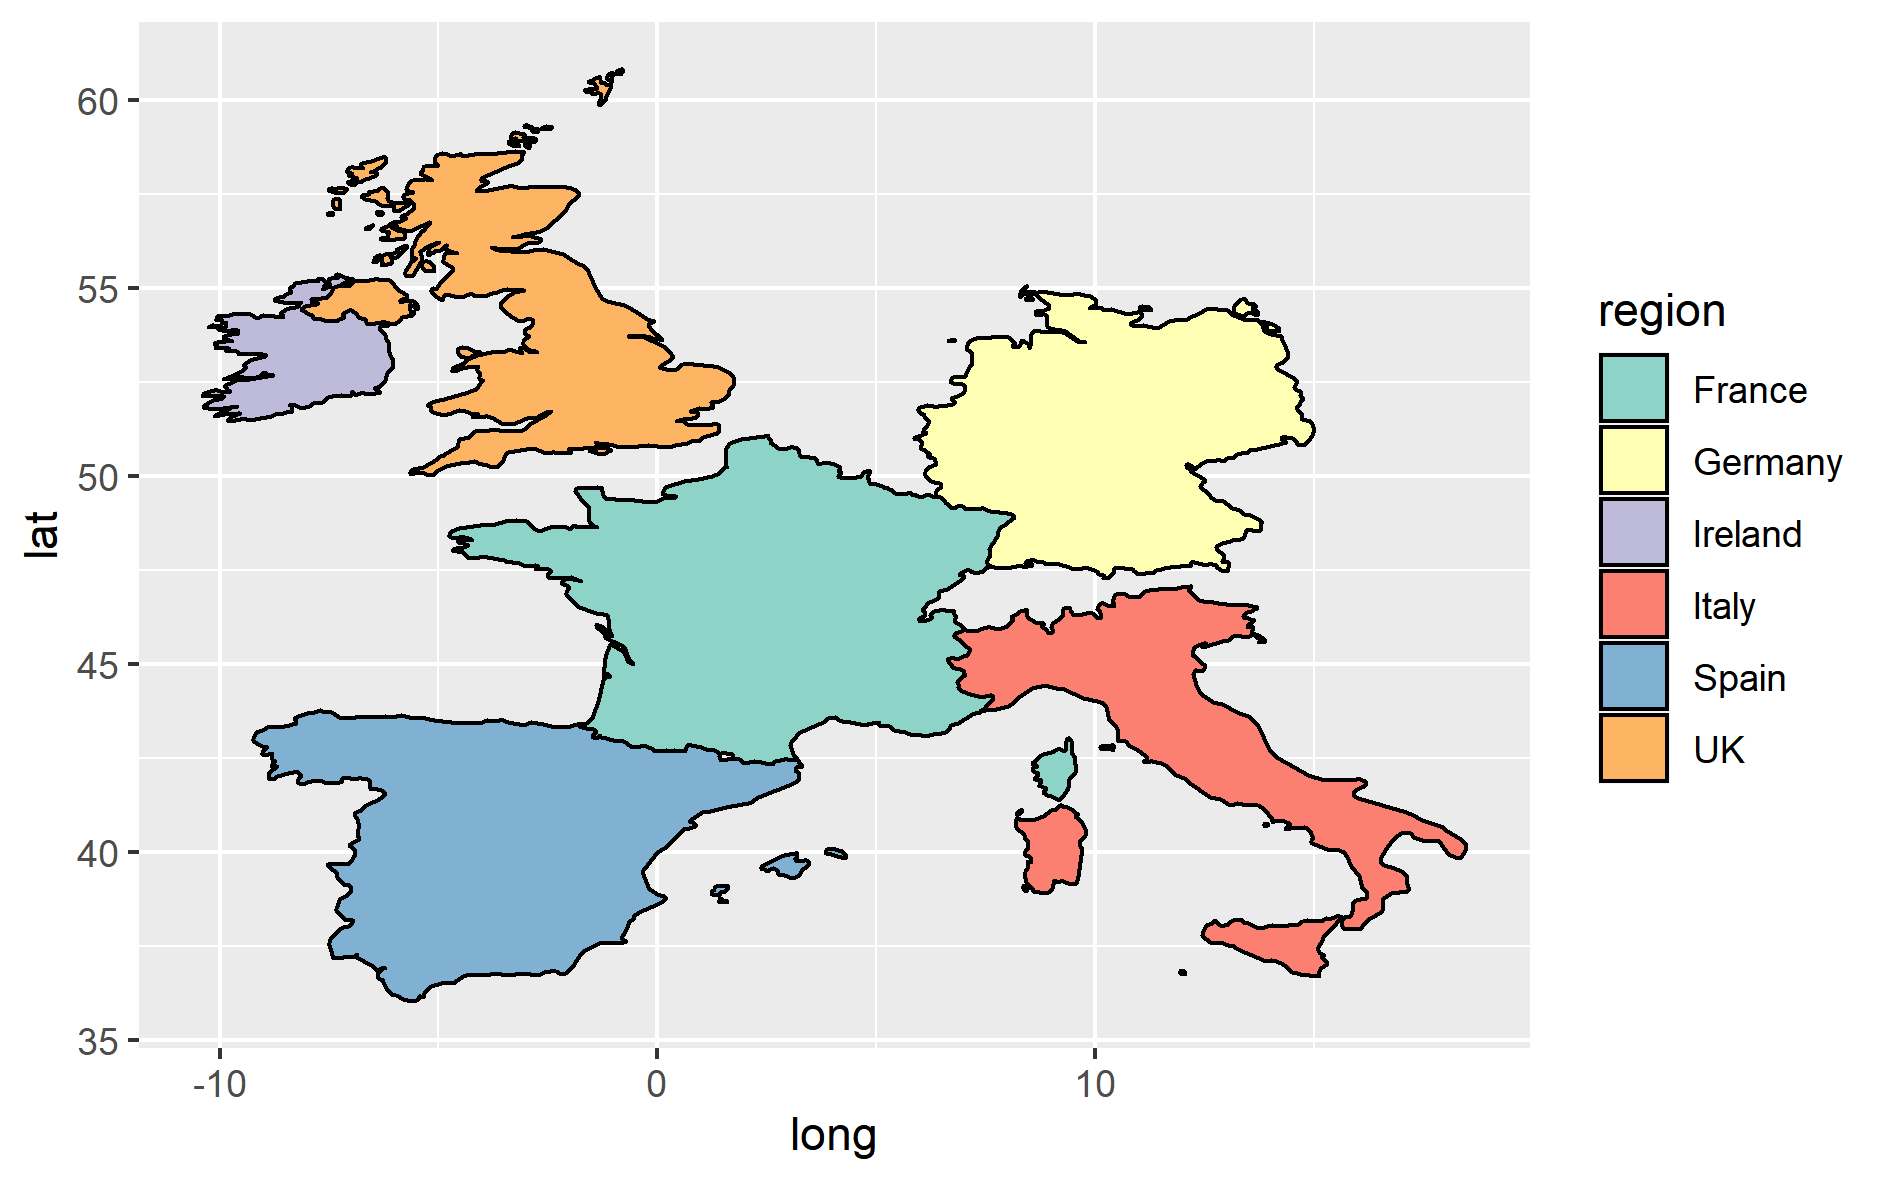
\includegraphics{original2.png}
\end{figure}
Para corregirlo, inclu\'imos en el gr\'afico las referencias, para identificar m\'as f\'acilmente cual es cada pa\'is. Para ello, inclu\'imos los centroides para obtener la posici\'on de las etiqueta. 

Para evitar que se expanda el gr\'afico al guardarlo con otras dimensiones, utilizamos una proyecci\'on particular (en este caso ``\texttt{gilbert}'' de manera arbitrar\'ia, tranquilamente podr\'iamos haber elegido ``\texttt{mercator}'').

Tambi\'en cambiamos el \textit{theme}. Agregamos t\'itulo, subt\'itulo y cambiamos las etiquetas de los ejes.

A continuaci\'on presentamos el resultado.
\begin{figure}[H]
    \centering
    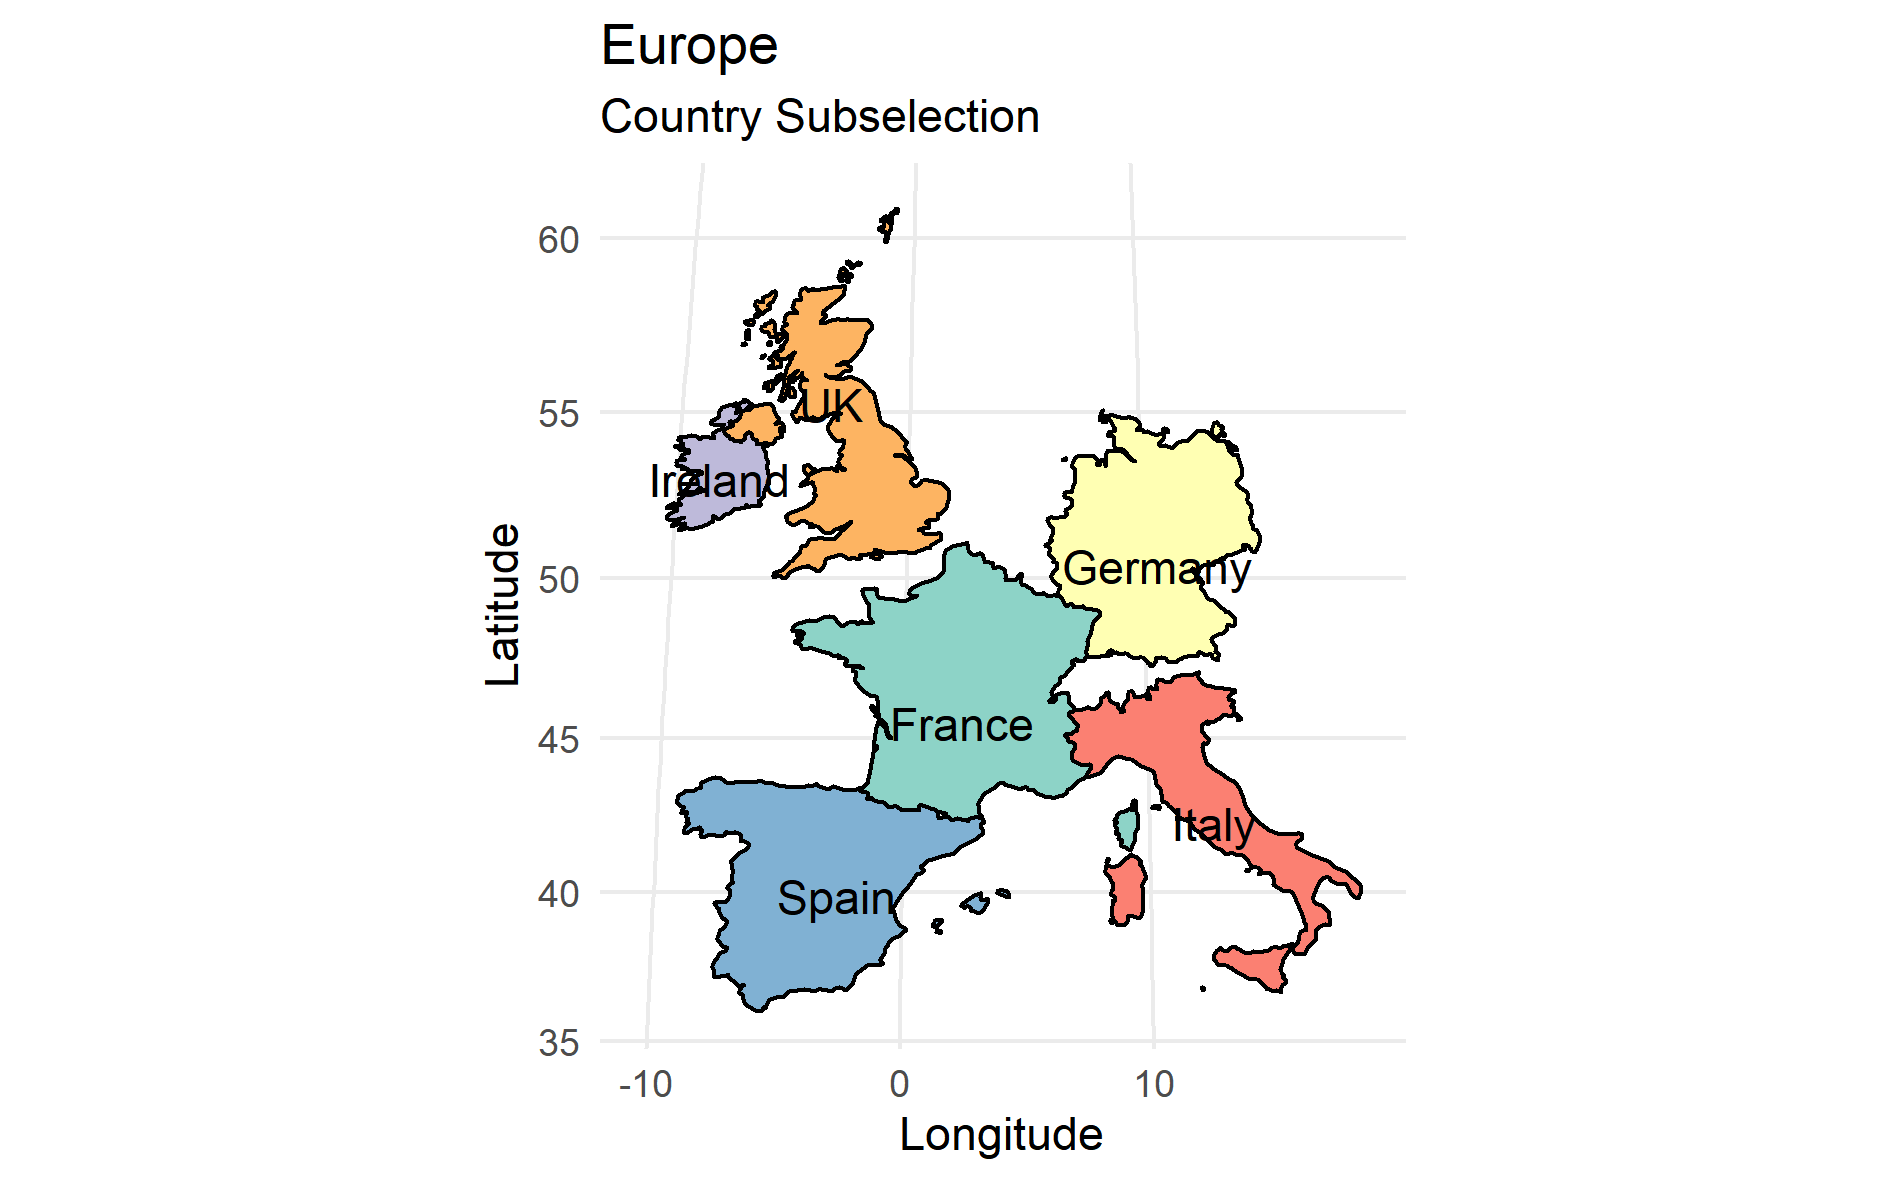
\includegraphics{changed2.png}
\end{figure}
\subsection*{Recaudaci\'on Bruta Mundial - Hollywood}
El siguiente gr\'afico (\texttt{p2}) presenta la recaudaci\'on bruta a nivel mundial de pel\'iculas de Hollywood en 2013 de distintos g\'eneros y estudios. A continuaci\'on el gr\'afico original.
\begin{figure}[H]
    \centering
    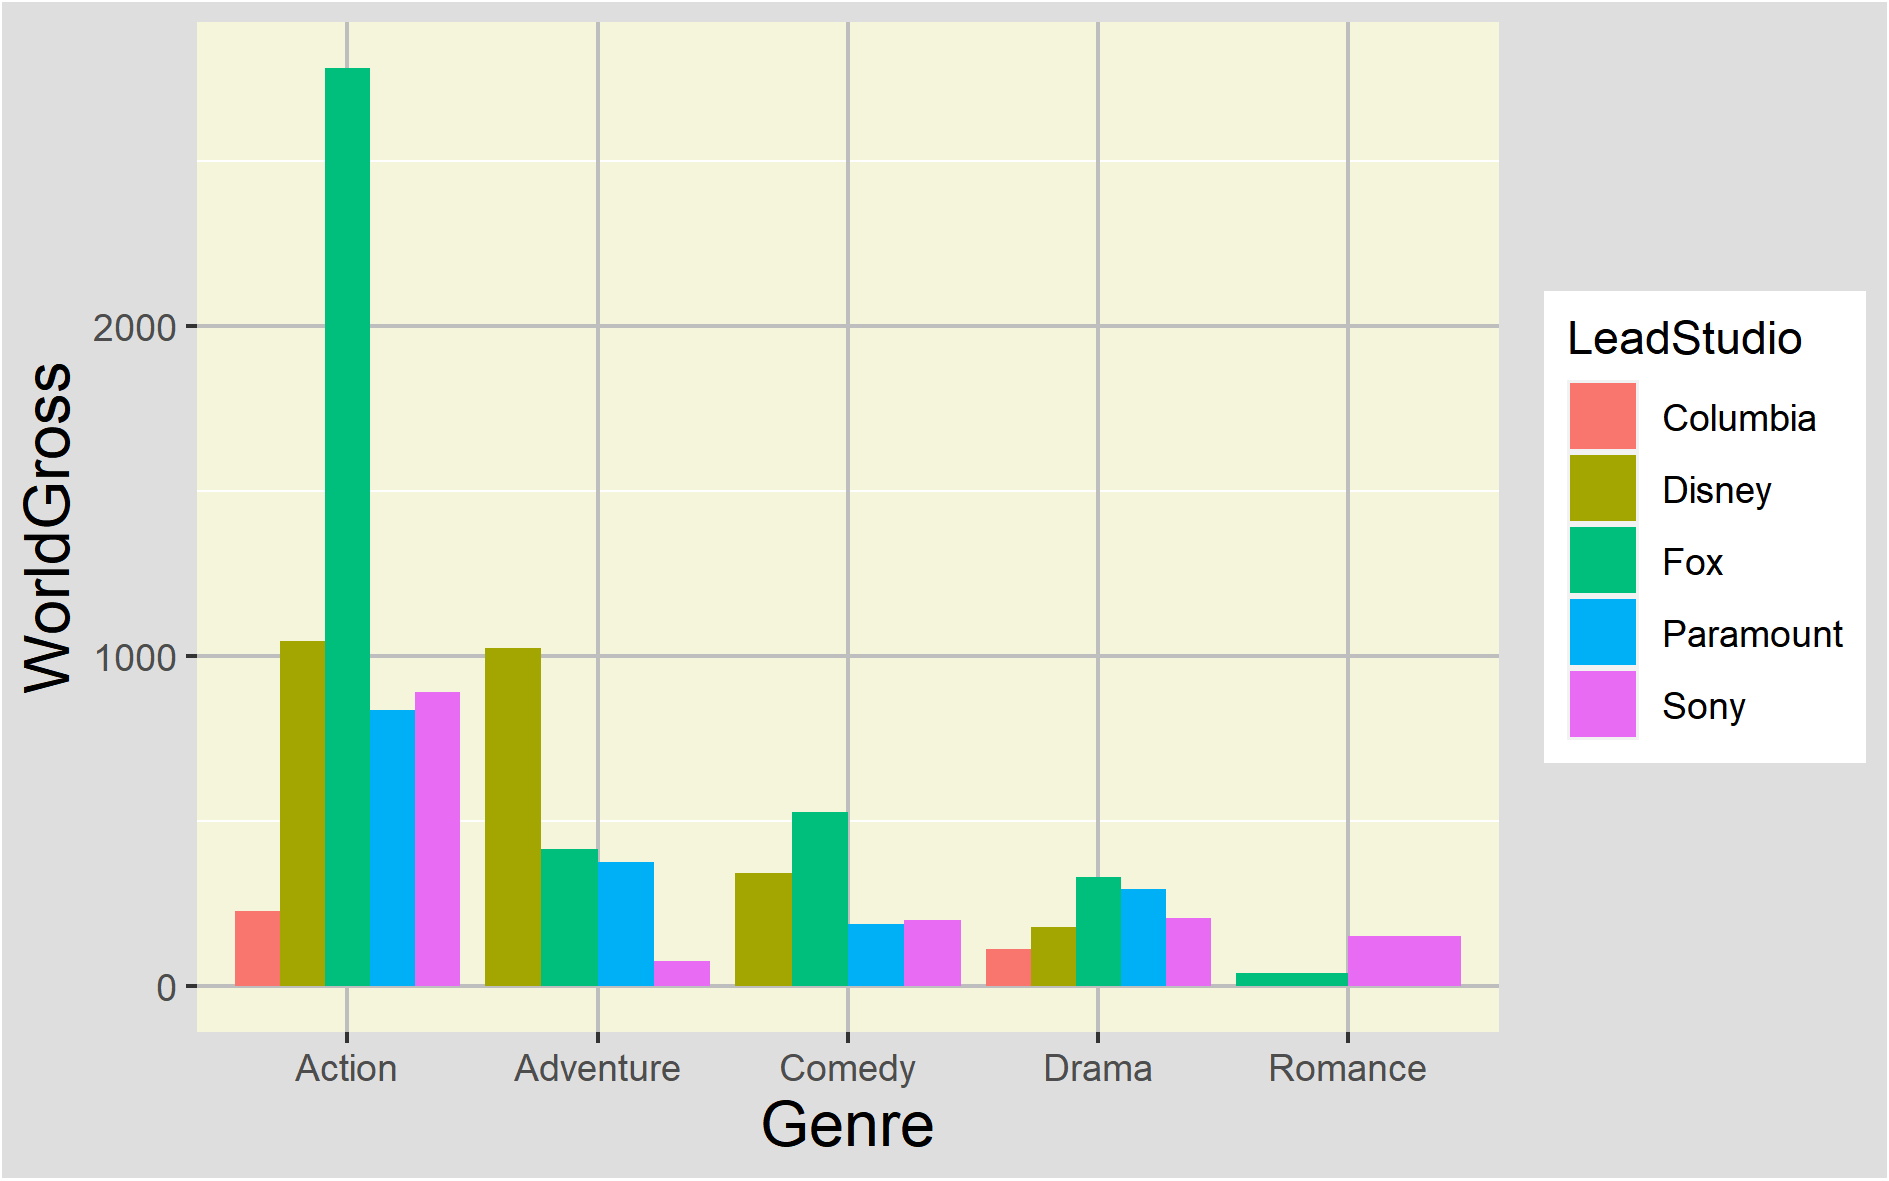
\includegraphics{original1.png}
\end{figure}
Nuevamente, homogeneizamos el \textit{theme} y paleta de colores con los dem\'as gr\'aficos. 

Entendiendo que importa la recaudaci\'on dividiendo por g\'enero, decidimos que l grafico de barras sea dividido por el g\'enero nom\'as. Luego, dividimos cada genero por estudio, pero apilado.

Con la intenci\'on de integrar la informaci\'on al cuadro, las etiquetas de estudio s eencuentran sobre la primer barra. 
Invertimos las coordenadas.
\begin{figure}[H]
    \centering
    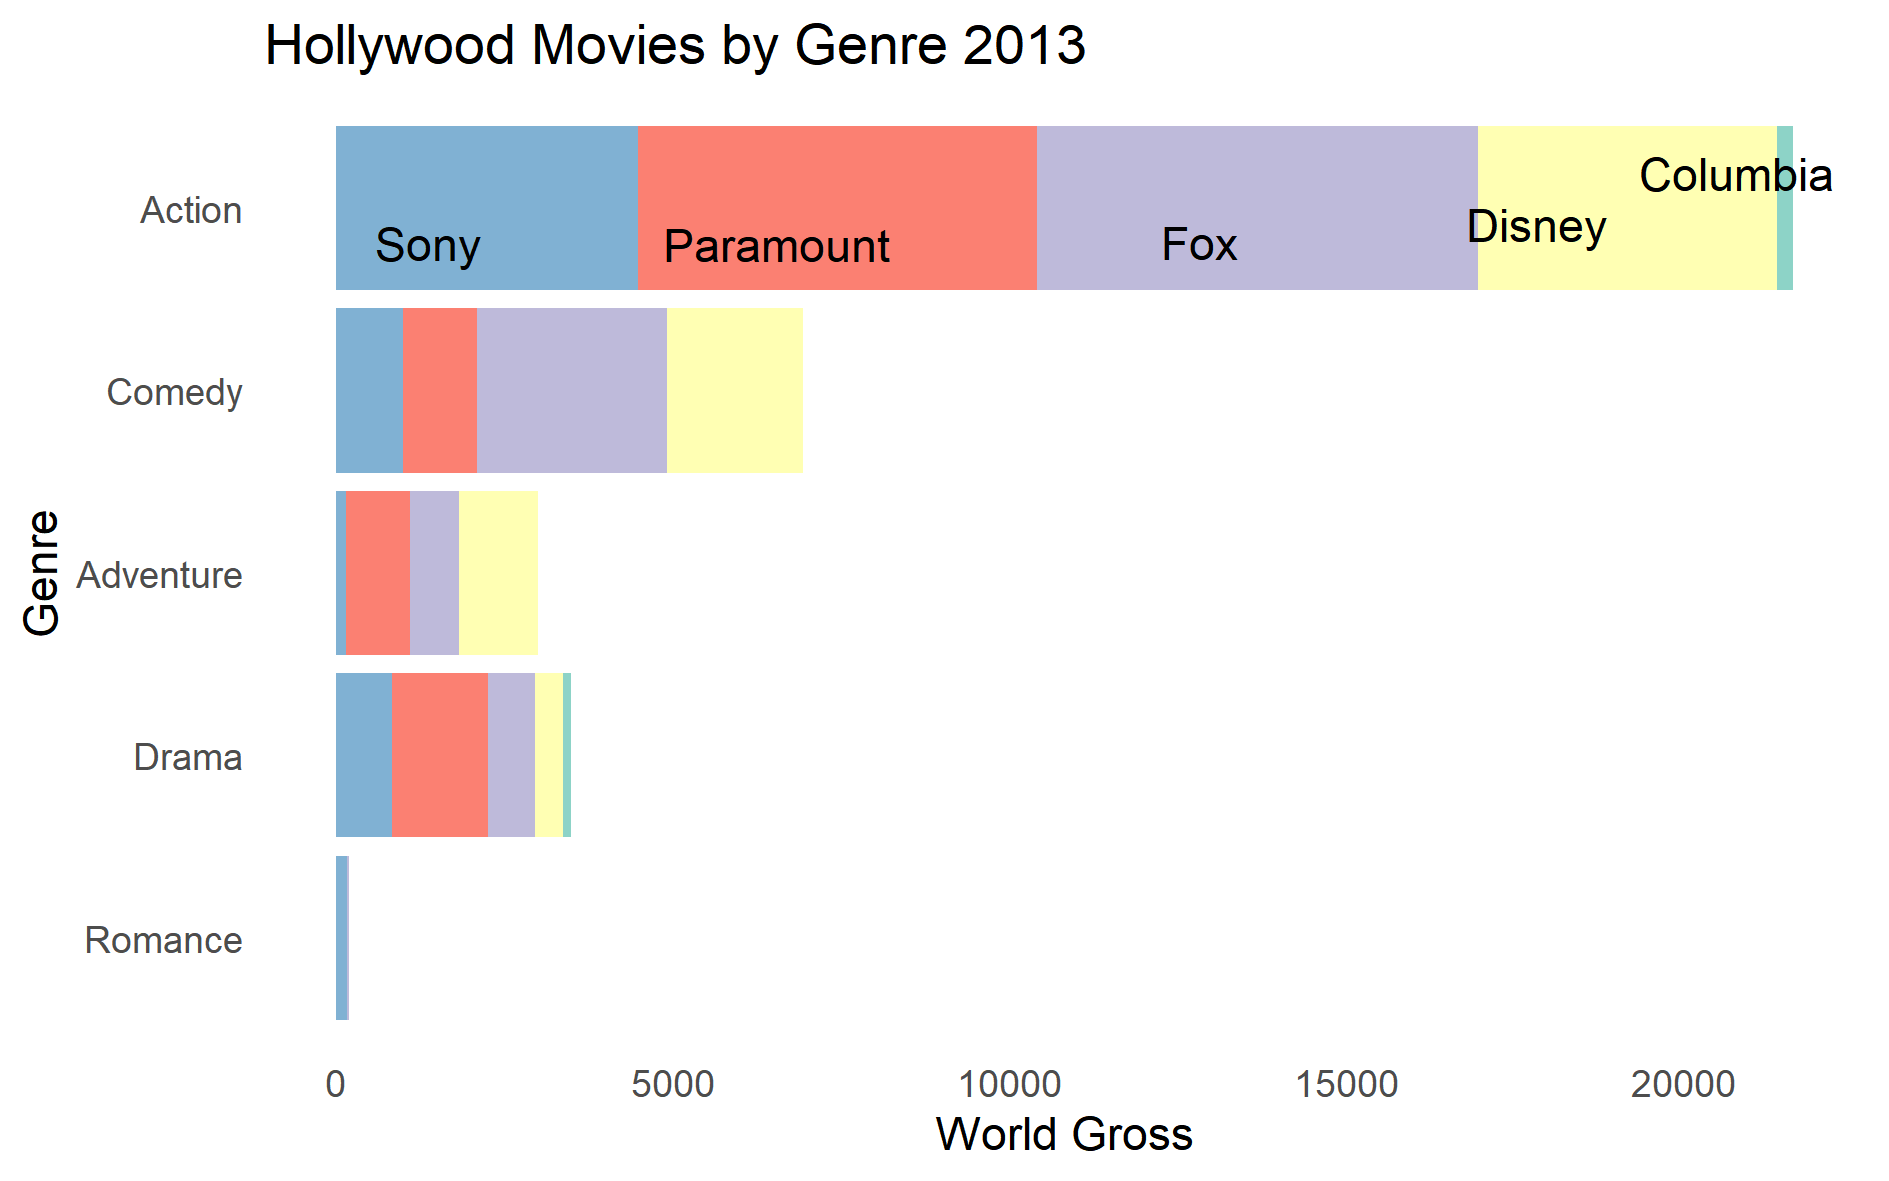
\includegraphics{changed1.png}
\end{figure}
\section*{Tarea 2}
Este ejercicio consiste en realizar con distintos paquetes en \texttt{R} y \texttt{STATA} el mismo gr\'afico: conteo de robos y hurtos en Londres para el per\'iodo 04/2011-03/2013 por distrito. Se puede notar que a medida que se acercan al centro, mayor es el conteo. Hay un distrito con falta de datos, mostr\'andose en gris: City of London.

Los colores en R son con un gradiente de colores. 

A continuaci\'on el mapa realizado con el paquete de \texttt{R tmap}:
\begin{figure}[H]
    \centering
    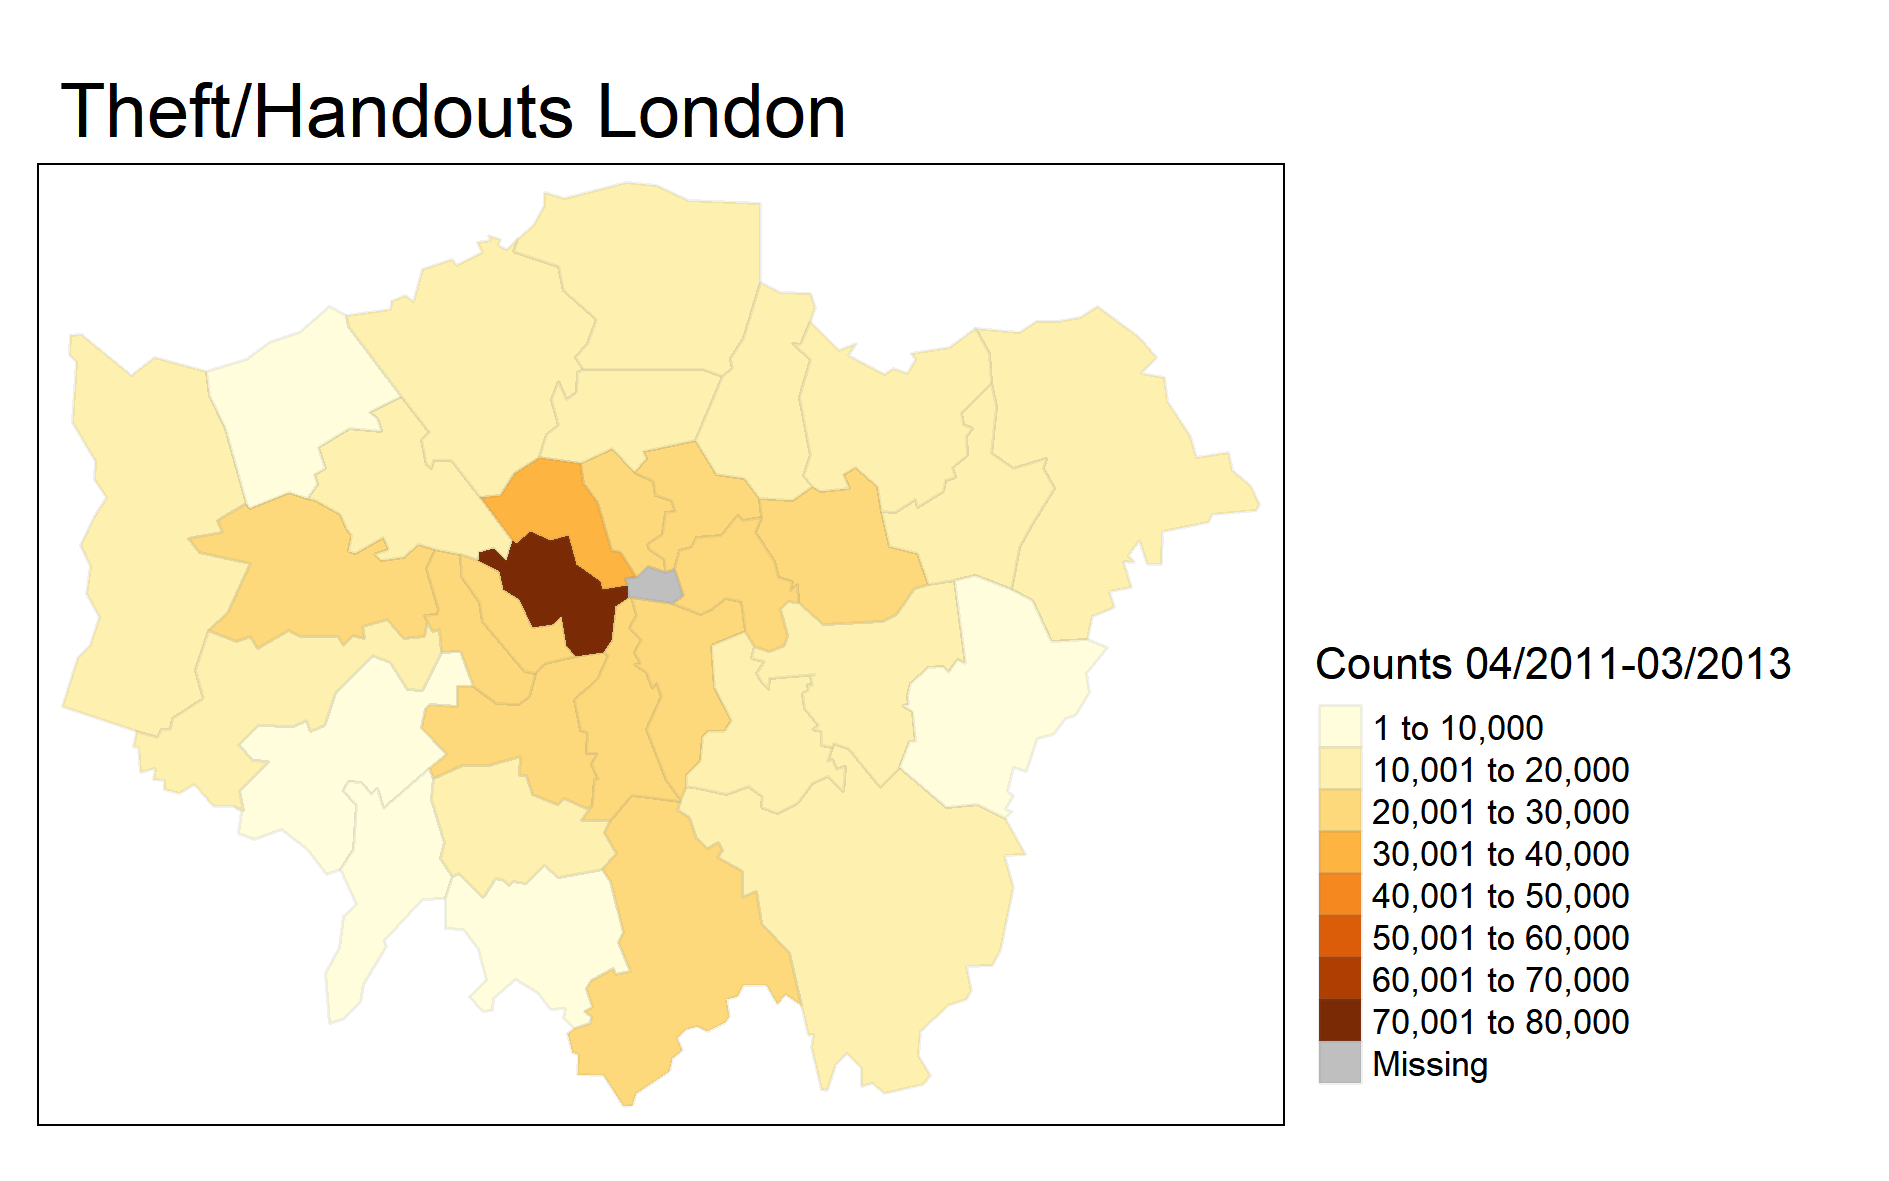
\includegraphics{thieftm.png}
\end{figure}
A continuaci\'on el mapa realizado con el paquete de \texttt{R ggplot2}.
\begin{figure}[H]
    \centering
    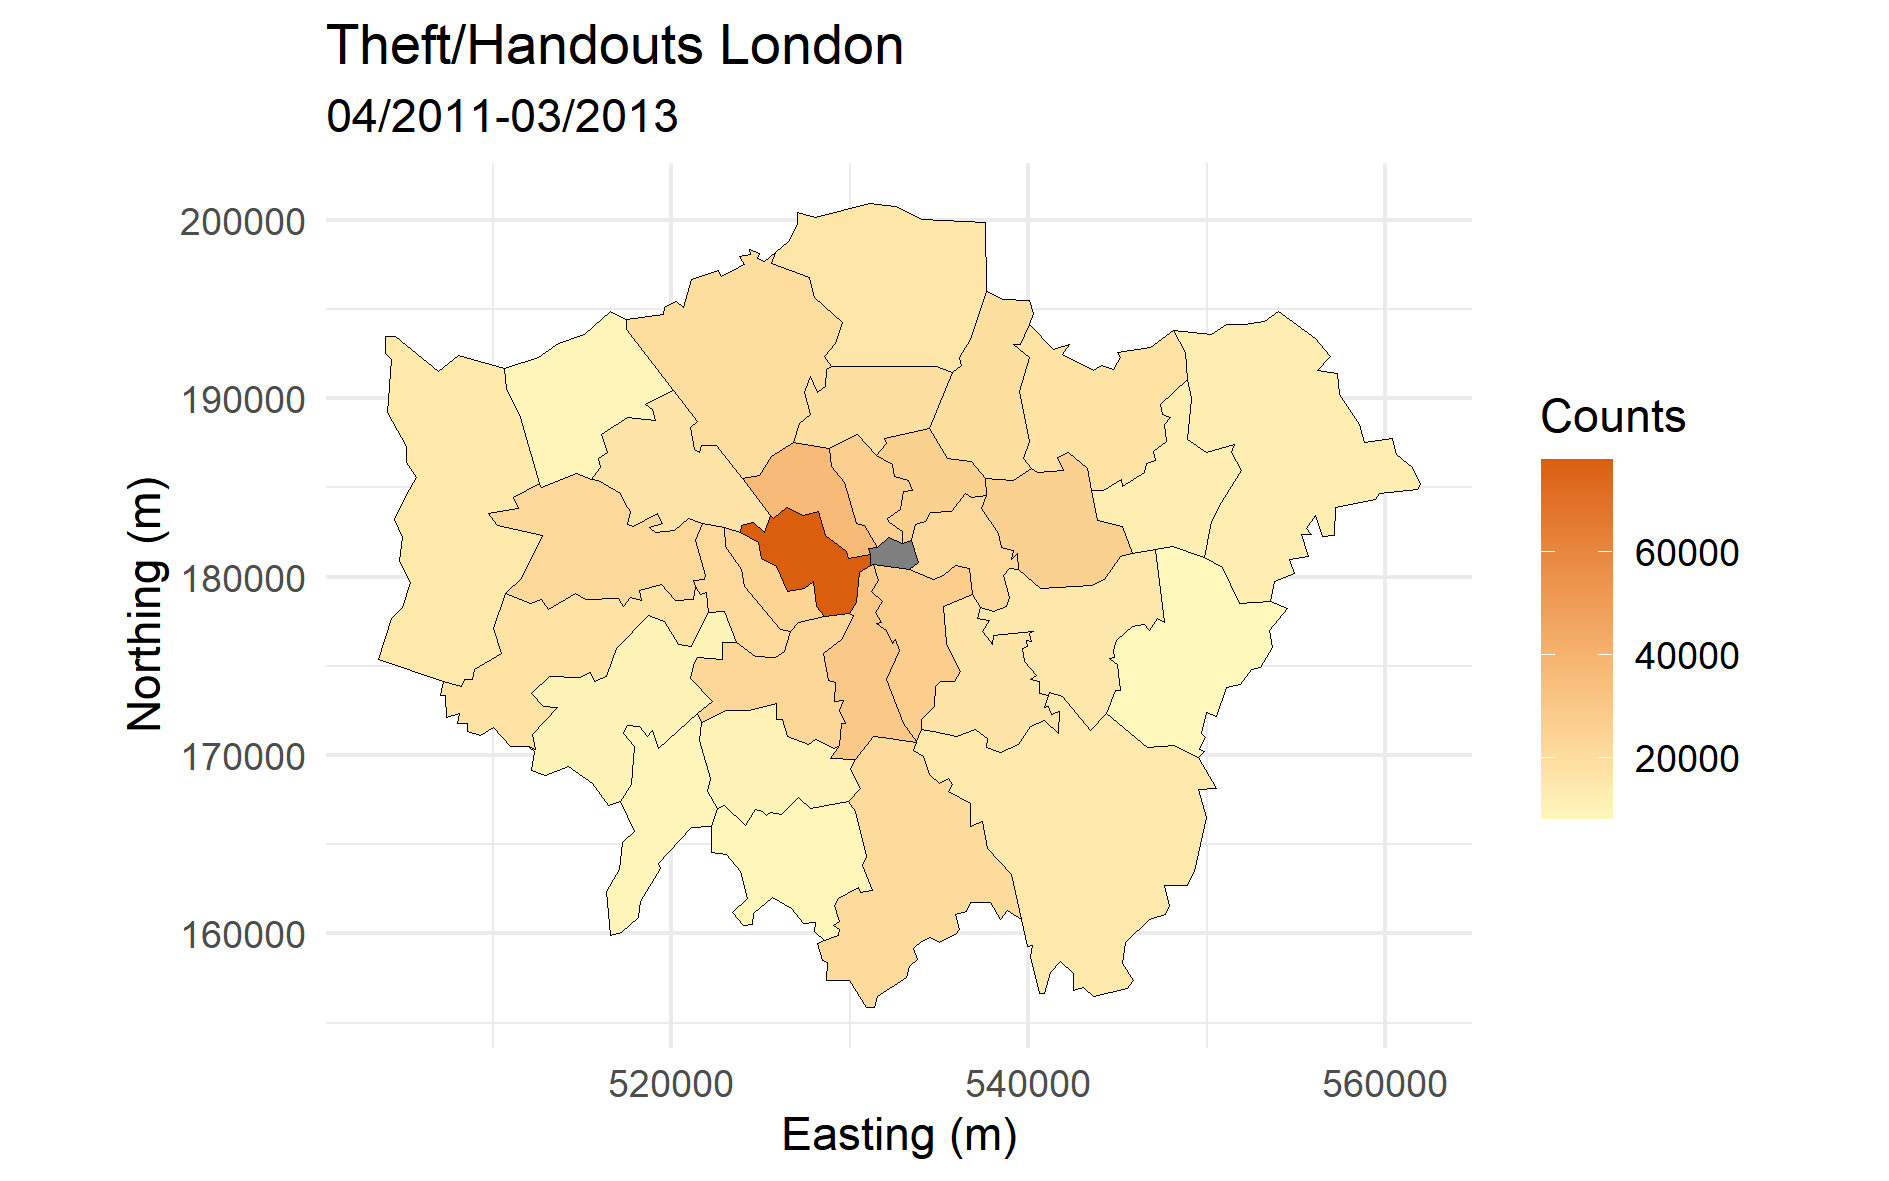
\includegraphics{thiefgg.png}
\end{figure}
Para el paquete de \texttt{STATA spmap}, utilizamos dos metodos distintos, ya que estos dividen los colores por intervalos. Primero, con intervalos equidistantes, resultando en un gr\'afico muy similares a los anteriores. 
\begin{figure}[H]
    \centering
    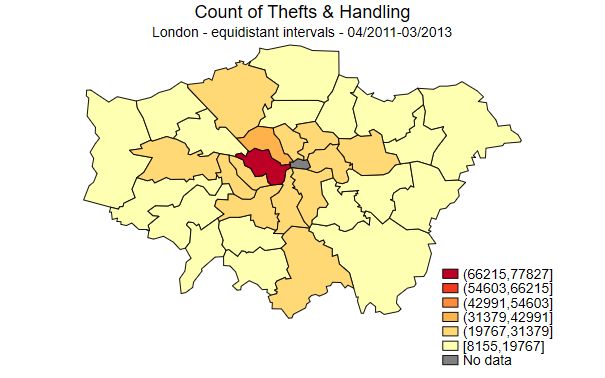
\includegraphics[width=0.85\textwidth]{theftspequidistant.png}
\end{figure}
Dividiendo los intervalos por quantiles, el gr\'afico resultante es el siguiente:
\begin{figure}[H]
    \centering
    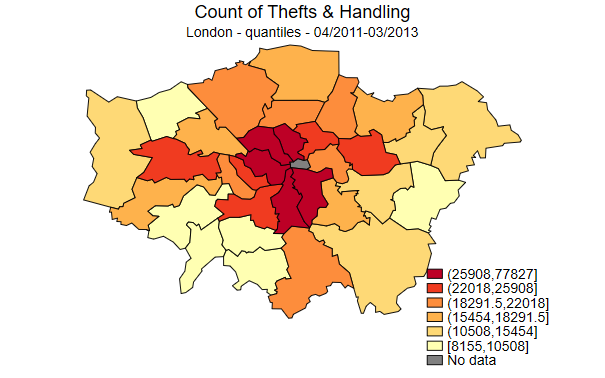
\includegraphics[width=0.85\textwidth]{theftspquantile.png}
\end{figure}
\end{document}
